\pagestyle{empty}
\cleardoublepage
\pagestyle{fancy}

%espaco entre linhas
\onehalfspacing

\chapter{Algoritmo Proposto}\label{cap4}

Esta seção demonstra detalhes de implementação do algoritmo proposto para o balanceamento de carga dinâmico em aglomerados de GPUs. 

Em uma típica aplicação paralela, os dados da aplicação são divididos entre as threads em um processo chamado decomposição de domínio. As threads então simultaneamente processam parte dos dados. Depois de terminarem, mesclam os resultados processados e terminam a aplicação ou continuam para a próxima fase de computação. A tarefa do algoritmo proposto é determinar o tamanho do bloco de dados atribuído a cada GPU e CPU no sistema. O termo processador significará uma única CPU ou GPU. Os processadores são diferentes entre si, o que torna o ambiente heterogêneo. 

O algoritmo apresenta três partes, que são: (1) modelo de desempenho do processador, onde um modelo de execução é determinado durante a execução da aplicação; (2) seleção do tamanho ótimo do bloco, onde baseado no modelo de performance no qual o algoritmo seleciona a melhor distribuição de tamanho de blocos entre os processadores; e (3) o rebalancemaento onde o algoritmo recalcula o tamanho do bloco ótimo quando a diferença no tempo de execução nos diferentes processadores é maior que um certo limiar.

O algoritmo inicialmente gera um modelo de desempenho do processador. Este modelo consiste em gerar curvas baseadas no desempenho do processador para uma dada tarefa. A curva consiste em fornecer um pedaço do problema a cada processador e determinar o tempo que o processador gastou para processar aquele pedaço do problema. Para cada processador uma curva é gerada, que representa o modelo de desempenho para aquele dado problema. O algoritmo Inicialmente determina a curva $P_p[x]$, que fornece a velocidade de processamento para um dado bloco de tamanho $x$ no processador $p$. Para construir estas curvas, um bloco de tamanho $initialBlockSize$, definido pelo usuário é atribuído para cada processador. Este tamanho inicial de bloco é arbitrário, e fica a cargo do usuário determina-lo.

Com o bloco de dados inicial igual para todos os processadores, é realizada a contabilização de todos os tempos. Este primeiro valor é o primeiro ponto utilizado para gerar a curva $P_p[x]$. O próximo ponto é determinado, elegendo o processador que realizou a tarefa em menor tempo, e dobrando o tamanho do bloco inicial para este processador. O restante dos processadores é realizado uma atribuição proporcional ao desempenho obtido na primeira atribuição. Supondo que o tempo do processador mais rápido seja $t_f$, dobra-se o tamanho do bloco para este processador. Para os outros processadores, com o tempo de término $t_i$, onde i é o tempo gasato para cada processador, seleciona-se o tamanho do bloco proporcional a razão $t_i/t_f$. 


\begin{figure*}[htb]
	\begin{center}
	\centering
			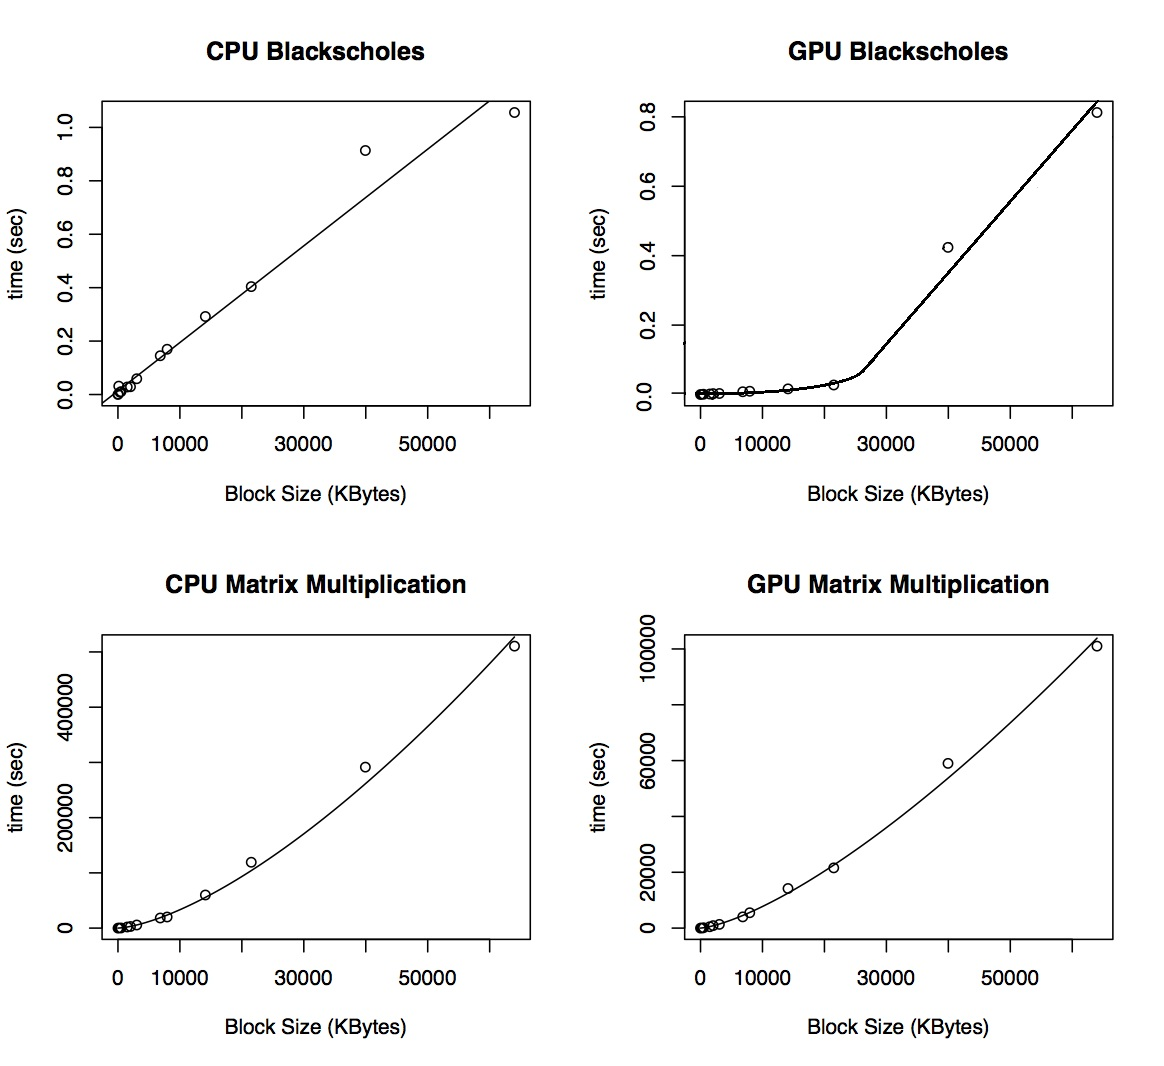
\includegraphics[scale=0.6]{CPUVersusGPULinear2.jpg}
	\caption{Curvas para GPU x CPU}
	\label{fig:CPUVersusGPU}
	\end{center}
\end{figure*}


A figura \ref{fig:CPUVersusGPU} mostra um exemplo de média de tempo para uma GPU e uma CPU para diferentes tamanhos de bloco. Pode-se notar que as curvas podem ser aproximadas por funções. Nestas curvas encontrou-se curvas que se ajustam através do método dos mínimos quadrados, usando uma função da forma $y= a_1f_1(x) + a_2f_2(x) + a_3f_3(x) + ... + a_nf_n(x)$. A curva é ajustada após a geração de poucos pontos, por exemplo quatro, gerando um modelo de tempo de execução para cada processador.

A figura \ref{fig:CPUVersusGPU} mostra um exemplo de medida de tempo de processamento para uma GPU e uma CPU para diferentes tamanhos de bloco em duas aplicações. Pode-se notar que as curvas para a aplicação blackscholes pode ser aproximada por funções lineares, enquanto para a multiplicação de matrizes usa-se uma função exponencial. Encontrou-se o melhor ajuste das curvas utilizando o método dos mínimos quadrados:

\begin{equation}
 y(x) = a_{1} f_{1}(x) +  a_{2} f_{2}(x) + ... + a_{n} f_{n}(x) 
\label{eq: least}
\end{equation} 

onde $f_i(x)$ corresponde ao seguinte conjunto de funções $x$, $x^2$, $x^3$, $e^x$, $ln x$ e seguintes combinações $xe^x$, $xlnx$. Se o modelo não se enquadrar em umas das funções descritas, é utilizada a função que aproxima o modelo. Os valores de $a_i$ são dados pelo próprio método dos mínimos quadrados, como valor de ajuste. O método dos mínimos quadrados testa para cada função e a que apresentar menor erro é a selecionada.

\begin{algorithm}

\caption{Modelo de desempenho do processador}
\label{algModel}

\begin{algorithmic}		

\STATE \textbf{function}~determineModel()

\STATE $blockSizeList \leftarrow initialBlockSize;$

\STATE $fitValues$ = determineCurveProcessor();

\WHILE {$iteration \neq 4$ }
		\STATE $finishTimes$ = executeTasks($blockSizeList$);
                \STATE synchronize();
	        \STATE $blockSizeList$ = evaluateNextBlockSizes($finishTimes$);
		\STATE $fitValues$ = determineCurveProcessor();
		\STATE $iteration++$;
\ENDWHILE

return $fitValues$;

\end{algorithmic}
\end{algorithm}

Os passos do algoritmo são mostrados em \ref{algModel}. A variável $blockSizeList$ contem o tamanhos dos blocos atribuídos a cada processador e é inicializada com $initialBlocoSize$, que é definida  pelo usuário. A variável $fitValues$ contem o resultado do ajuste por mínimos quadrados, incluindo o erro no ajuste, que é inicializado como $+\infty$. 

O laço é limitado a 4 pontos para gerar a curva. A função envia um pedaço de dados para cada processador e obtêm o tempo que demorou para realizar o processamento em cada processador. Depois de esperar, que todos os processadores terminem, é determinado o tamanho do bloco para a próxima iteração, baseado no tempo de término de cada processador. Por fim, o algoritmo tenta ajustar um modelo de curva para cada processador e recebe o resultado do ajuste.

\textit{Seleção do tamanho de bloco ótimo:} O algoritmo determina o tamanho do bloco ótimo para cada processador com o objetivo de minimizar o  tempo total da aplicação. Considere que existem $n$ processadores e o tamanho da entrada seja $Z$. O algoritmo atribui um pedaço de dados de tamanho $x^g$ para cada processador $g= 1,..., n$, correspondendo a uma fração dos dados de entrada, tal que $\sum_{g=1}^n x^g = Z$. Denota-se como $E^g(x^g)$ o tempo de execução da tarefa $E$ no processador $g$, para cada entrada de tamanho $x^g$. Para distribuir o trabalho entre os processadores, encontra-se um conjunto de valores:

\begin{equation}
	X = \{ x^g \in \mathbb{R}:[0,1] / \sum_{g=1}^n x^g = Z \}
	\label{eq: totalResultado}
\end{equation}

que minimiza $E^1(x^1)$ enquanto satisfaz a restrição:

\begin{equation}
	E^{1} = E^{2} = ...= E^{n}
	\label{eq: Restricao}
\end{equation}
 
que representa que todos os processadores gastariam uma mesma quantidade de tempo realizando o processamento. Para determinar o conjunto de valores de $x$, resolve-se o sistema de equações das curvas ajustadas para todos os processadores, dados por:

\begin{equation}
	\left\lbrace
	\begin{array}{ll}
		\displaystyle E_{1} = Y^1(x_{1})  \\
		\displaystyle E_{2} = Y^2(x_{2})   \\
		\displaystyle E_{n} = Y^n(x_{n}) 
		\label{eq: system}
	\end{array}
	\right.
\end{equation}

O sistema de equações é resolvido aplicando  \emph{interior point line search filter method}. O algoritmo busca minimizar as funções no espaço de busca. Ele alcança uma solução ótima percorrendo o interior de uma solução viável. Determinar o valor de $x$ tal que o tempo é mínimo. A complexidade do método é sempre polinomial.

\textit{Rebalanceamento:} Depois de resolver o sistema de equações o escalonador mantem enviando tarefas de tamanho $x_i$ para cada processador $i$, logo que o processador termina a tarefa anterior. Também monitora o tempo de término de cada tarefa. Se a diferença no tempo de término entre $x_i$ e $x_j$ de qualquer duas tarefas $i$ e $j$ for maior que um limiar, o processo de balanceamento é reexecutado. Neste caso, o algoritmo aplica o modelo de desempenho e a rotina de determinação do tamanho do bloco ótimo novamente. O escalonador então sincroniza as tarefas e inicia usando o novo valor de $x_i$. O limiar ($\alpha$) precisa ser determinado empiricamente através de alguns testes, apenas roda-se a aplicação com valores entre 0.1 e 1. Se o limiar é um valor muito pequeno, ocorre balanceamentos desnecessários, que aumentará o tempo total da aplicação. Se o limiar é muito grande balanceamento necessários podem não ocorrer, o que pode fazer com que threads fiquem ociosas.

\begin{figure}[!t]
	\centering
			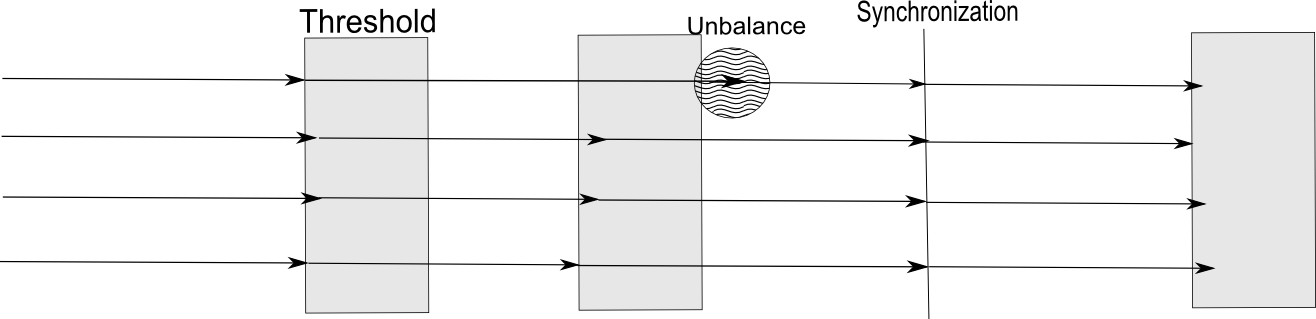
\includegraphics[scale=0.24]{DiagramaArtigo.png}
	\caption{Execução das Threads com limiar}
	\label{fig:Diagrama}
\end{figure}

A figura \ref{fig:Diagrama} apresenta um diagrama de execução para quatro threads e uma thread desbalanceada. As caixas representam os limiares, as linhas as threads e os círculos o desbalanceamento. As threads iniciam sincronizadas, recebem carga, mas em um segundo passo uma thread leva mais tempo que o valor de limiar, isto causa o desbalanceamento. Detectado o desbalanceamento, todas as threads são sincronizadas, e as partes são recalculadas para cada thread, fazendo com que as threads voltem ao estado de término dentro do valor de limiar estabelecido.



\begin{algorithm}

\caption{Algoritmo Dinâmico Completo}
\label{alg1}

\begin{algorithmic}		

\STATE \textbf{function} dynamic()

\STATE $fitValues$ = determineModel()
\STATE $X$ = solveEquationSystem($fitValues$);

\WHILE{there is data}

	\STATE $finishTimes$ = executeTasks($X$);
	\IF {$ $maxDifference($finishTimes$)$ \geq threshold$}
		\STATE $fitValues$ = determineModel();
                \STATE $X$ = solveEquationSystem($fitValues$);
                \STATE synchronize();
    	\ENDIF
\ENDWHILE

\end{algorithmic}
\end{algorithm}

Algoritmo Completo: Algoritmo \ref{alg1} apresenta o pseudocódigo do algoritmo de escalonamento. A função $determineModel$ mostrada no algoritmo \ref{algModel} retorna o modelo de desempenho para cada processador. Então resolve o sistema de equações para determinar a melhor distribuição de pedaços de dados para cada processador. Optou-se por não calcular a todo instante o modelo, para não aumentar o tempo gasto com o balanceamento de carga.

O laço inicial repete enquanto há dados ainda para serem processados. É distribuído pedaços de dados para cada processador do sistema, obtendo o tempo de término para cada execução de tarefa. É checado se a diferença máxima entre o término das tarefas está acima de um limar, obtido empiricamente. Se o limiar é alcançado, o algoritmo ajusta um novo modelo de curvas e resolve o sistema de equações para estas novas curvas para determinar uma nova distribuição de tamanhos pedaços de dados.

 
	










